\documentclass{beamer}
\usepackage{epstopdf}
\usepackage{tikz}
\usepackage{tabu}
\usepackage{adjustbox}
\usepackage{graphicx}
\usepackage{tabularx}
\usepackage{multirow}
\usepackage{booktabs}
  \setbeamertemplate{mini frames}{}
  % or ...

\usepackage{hyperref}
\usepackage{pgf,pgfarrows,pgfnodes,pgfpages}
\usepackage[english]{babel}

\usepackage[latin1]{inputenc}

\title[] % (optional, use only with long paper titles)
{\vskip0pt\normalsize{USDA Food Assistance Programs (SNAP, the National School Lunch Program, and the School Breakfast Program) and Healthy Food Choices: Quasi-Experimental Evidence from Geographic Variation in Food Prices}}

\subtitle
{} % (optional)

\author%[Author, Another] % (optional, use only with lots of authors)
{\small{{Erin Todd Bronchetti (Swarthmore College) \\ Garret Christensen (UC Berkeley)\\ Benjamin Hansen (University of Oregon)}}}
% - Use the \inst{?} command only if the authors have different
%   affiliation.

\date[Short Occasion] % (optional)
{November 2017* \\
Preliminary: Please check before citing}


\subject{Talks}
%\titlegraphic{\includegraphics[width=\textwidth,height=.5\textheight]{nudgebanner}}

% If you wish to uncover everything in a step-wise fashion, uncomment
% the following command: 

%\beamerdefaultoverlayspecification{<+->}
%\titlegraphic{\includegraphics[width=\textwidth,height=.5\textheight]{someimage}}
%\begin{beameroption}{show only notes{}
\def\tiny{\fontsize{7pt}{7pt}\selectfont}
\setbeamerfont{section in head/foot}{size=\tiny}

\begin{document}

\begin{frame}
  \titlepage
 
  \tiny{\begin{quote}This project was supported with grants from the National Bureau of Economic Research and University of Kentucky Center for Poverty Research through funding by the U.S. Department of Agriculture, Economic Research Service and the Food and Nutrition Service, Agreement Numbers 58-5000-1-0050 and 58-5000-3-0066. The opinions and conclusions expressed herein are solely those of the author(s) and should not be construed as representing the opinions or policies of the sponsoring agencies\end{quote}}
%\note[item]<1>{Thank you all for being here today, during this very busy first week of classes.}
%\note[item]<1>{I, personally, am delighted to be beginning another academic year at Swarthmore...}
%\note[item]<1>{"Portfolio approach" ... projects in several different topic areas ... all connected by an interest in social welfare policy and social insurance...} 
%\note[item]<1>{as well as a focus not just on the COSTS of these programs (incentive effects)... but also on the BENEFITS -- (protect material wellbeing)}
  %\end{singlespacing}
   %\end{reference} 
\end{frame}

%\newcounter{saveenumi}
%\newcommand{\seti}{\setcounter{saveenumi}{\value{enumi}}}
%\newcommand{\conti}{\setcounter{enumi}{\value{saveenumi}}}

%\begin{frame}{Outline}
  %\tableofcontents
  % You might wish to add the option [pausesections]
%\end{frame}


\begin{frame}
\begin{figure}
\frame{

\includegraphics[scale=0.25]{./images/1200px-Supplemental_Nutrition_Assistance_Program_logo.png}}

Slides available at 

\small{
\url{http://www.github.com/garretchristensen/FoodAPSAPPAM2017}}
\end{figure}

\end{frame}


\begin{frame}{Outline}
\begin{itemize}
\item SNAP Background
\item Food Price Variation Background
\item SNAP Sufficiency
\item Nutrition: Methods
\item Nutrition: Results
\item Conclusion
\end{itemize}
\end{frame}
%%%%%%%%%%%%%%%%%%%%%%%%%%%%%%%%%%%%%%%%%%%%%%%%%%%%%%%%%%%%%%%%%%%%%%%%%%%%%%%%%%%%%%
\section{Introduction}

\begin{frame}{SNAP Background}
The Supplemental Nutrition Assistance Program (SNAP) is one of the largest government assistance programs.
\begin{itemize}
\item
	2016: 44m recipients, cost of \$70 billion FY2016 
	
	\begin{tiny}[\href{https://fns-prod.azureedge.net/sites/default/files/pd/SNAPsummary.pdf}{Source: USDA FNS}]
\end{tiny}	
\item 
	Started in 1964%, expanded in 1971, purchase requirement eliminated in 1977
\item 
	Paid for by Feds (the farm bill), administered by states
\item
	Electronic Balance Transfer (EBT) in early 2000s
\item 
	Name changed to SNAP in 2008.
\end{itemize}
\end{frame}

\begin{frame}{How It Works}
Eligibility:
\begin{itemize}
\item Less than \$2,250/\$3,500 in countable assets. (Not home, sometimes car.)
\item Less than net monthly income 100\% of FPL, Gross 130\% (\$2,021/\$2,628 family of 4)
\item Earned income, dependent care, medical expenses, child support, excess shelter deductions.
\item $ Benefits=MaxBenefits(\$649/month)-NetIncome*0.3 $
\end{itemize}
\begin{tiny}
\href{https://www.fns.usda.gov/snap/eligibility}{[Source:USDA FNS]}
\end{tiny}
\end{frame}



\begin{frame}{Recent Issues}
\begin{itemize}
\item Large increase in recipients after financial crisis.
\item ARRA: Benefits increased \$80/month in 2009, decreased in 2013.
\item Able bodied without dependents 18-49(ABAWDs) eligibility maxes out at 3/36 months. Waived with high unemployment---kicking back in after Great Recession.
\item Food insecurity among recipient households remains quite high \href{http://www.ers.usda.gov/media/1896841/err194.pdf}{(Coleman-Jensen et al., 2014)}.
\end{itemize}
\end{frame}

\begin{frame}{Very Recent Issues}
Administration Proposals:
\begin{itemize}
\item \$193b (25+\%) cut over 10 years
\item Require ABAWDs work if $<$10\% unemployment
\item Eliminate minimum benefit (\$16)
\item Eliminate increase in benefits beyond 6 people in household. 
\end{itemize}
\begin{tiny}
\href{https://www.cbpp.org/research/food-assistance/presidents-budget-would-shift-substantial-costs-to-states-and-cut-food}{[Source: CBPP]}
\end{tiny}
\end{frame}

\begin{frame}
\begin{figure}
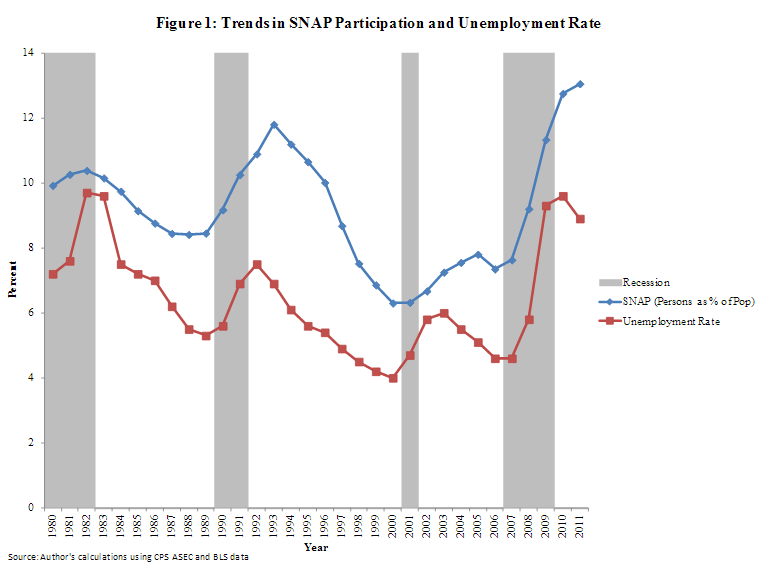
\includegraphics[width=\textwidth]{./images/Ziliak.PNG}

\href{http://gattonweb.uky.edu/Faculty/Ziliak/Ziliak_SNAP_100413.pdf}{Ziliak 2015, ``SNAP Matters''}
\end{figure}
\end{frame}

\begin{frame}{Our Research I}
\begin{itemize}
\item
 While legislated maximum SNAP benefits are fixed across 48 states, food prices vary significantly across geographic locations.
\item Deductions for costs of housing, medical care, and dependent care help may not be sufficient to equalize real value of SNAP benefits geographically.
\begin{itemize}
\item Small scale study in Philadelphia \href{http://www.childrenshealthwatch.org/publication/real-cost-of-a-healthy-diet-2011/}{(Breen et al., 2011)}.
\item  Quarterly Food at Home Price Database \href{http://www.ers.usda.gov/data-products/quarterly-food-at-home-price-database.aspx}{(QFAHPD)} price variation (35 market groups) shows  a \$10 increase in food price leads to 2.7 percentage point (5\%) increase in household food insecurity. (3.1 pp, 12\% for children) \href{http://aepp.oxfordjournals.org/content/35/4/679}{(Gregory \& Coleman-Jensen, 2013)}.
\end{itemize}
\end{itemize}
\end{frame}

\begin{frame}{Our Research II}
\begin{itemize}
\item
 What fraction of recipients can actually afford the TFP locally?
\item 
\textbf{What does SNAP relative generosity do to nutrition?}
\begin{itemize}
\item Literature: SNAP overall leads to modest changes in diet quality \href{https://www.ers.usda.gov/webdocs/publications/45059/36939_err147.pdf?v=41388}{(Gregory et al. 2014).}
\end{itemize}
\vskip0.25in
\item Other data (QFAPHD): 
 What does SNAP relative generosity do to child health? (Bronchetti, Christensen, Hoynes)
\end{itemize}
\end{frame}

%%%%%%%%%%%%%%%%%%%%%%%%%%%%%%%%%%%%%%MAPS%%%%%%%%%%%%%%%%%%%%%%%%%%%%%%%%%%%%%%%%%

{
   \setbeamertemplate{navigation symbols}{}
    \begin{frame}[plain]
        \begin{tikzpicture}[remember picture,overlay]
            \node[at=(current page.center)] {
                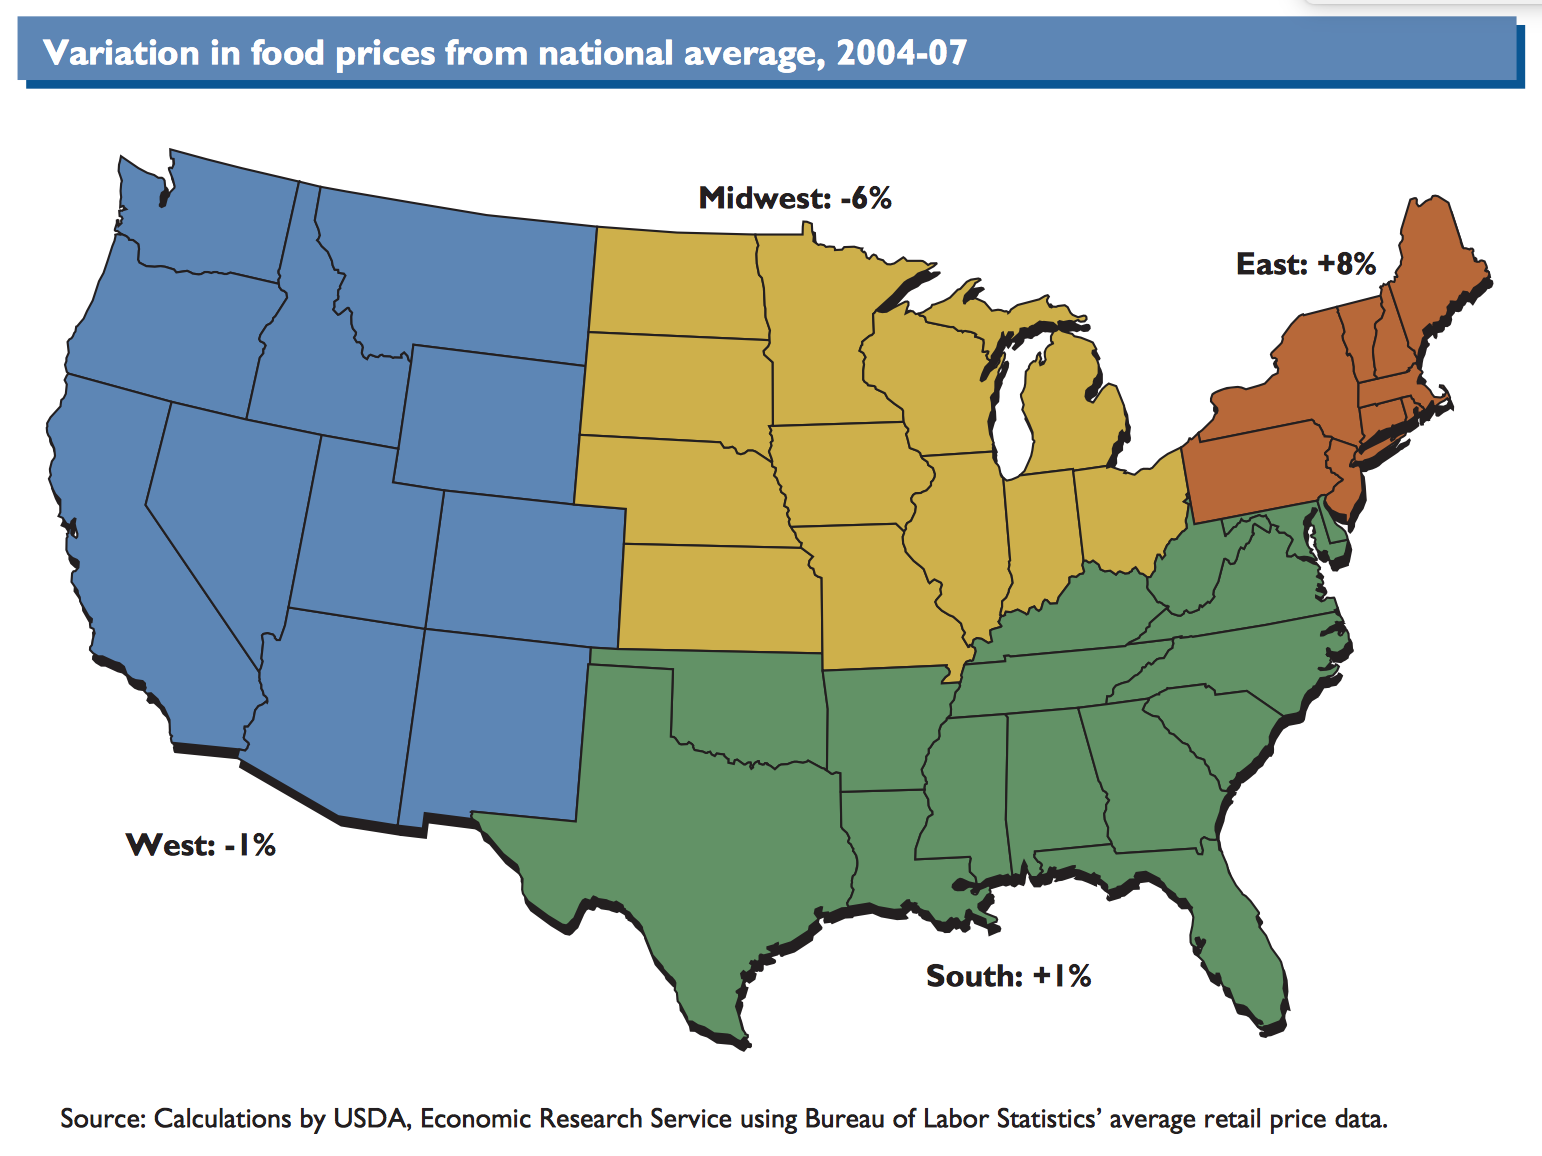
\includegraphics[width=\paperwidth]{./images/region_FPvary_map.png}
            };
        \end{tikzpicture}
     \end{frame}
}

{
   \setbeamertemplate{navigation symbols}{}
    \begin{frame}[plain]
        \begin{tikzpicture}[remember picture,overlay]
            \node[at=(current page.center)] {
                \href{http://www.ers.usda.gov/publications/eib-economic-information-bulletin/eib29-2.aspx}{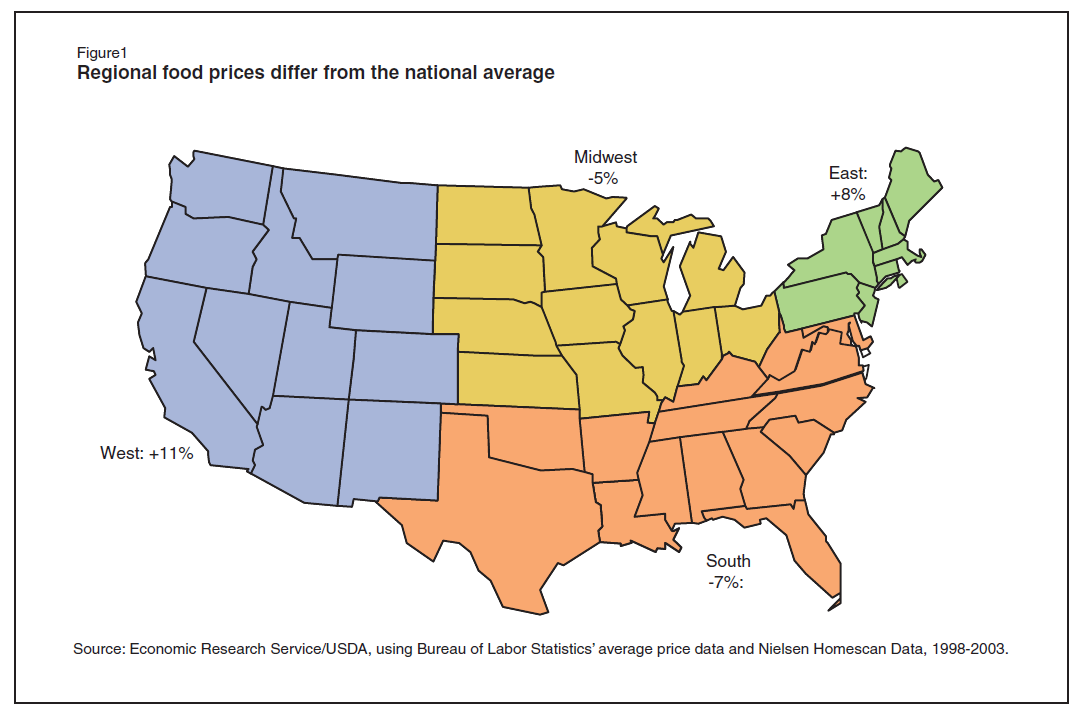
\includegraphics[width=\paperwidth]{./images/region_FPvary_map2.png}}
            };
        \end{tikzpicture}
     \end{frame}
}

{
   \setbeamertemplate{navigation symbols}{}
    \begin{frame}[plain]
        \begin{tikzpicture}[remember picture,overlay]
            \node[at=(current page.center)] {
                \href{http://www.ers.usda.gov/media/176139/page19.pdf}{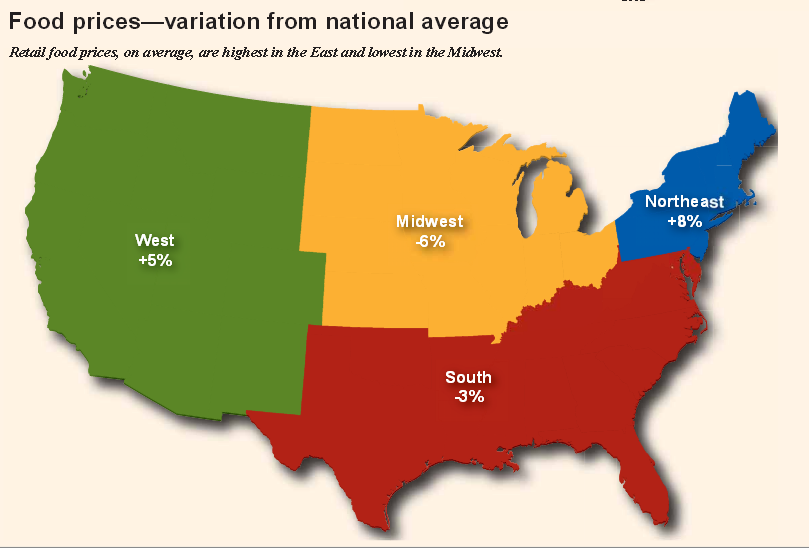
\includegraphics[width=\paperwidth]{./images/region_FPvary_map3.png}}
            };
        \end{tikzpicture}
     \end{frame}
}

%%%%%%%%QFAHPD
{
   \setbeamertemplate{navigation symbols}{}
    \begin{frame}[plain]
        \begin{tikzpicture}[remember picture,overlay]
            \node[at=(current page.center)] {
                \href{http://www.ers.usda.gov/publications/tb-technical-bulletin/tb1926.aspx}{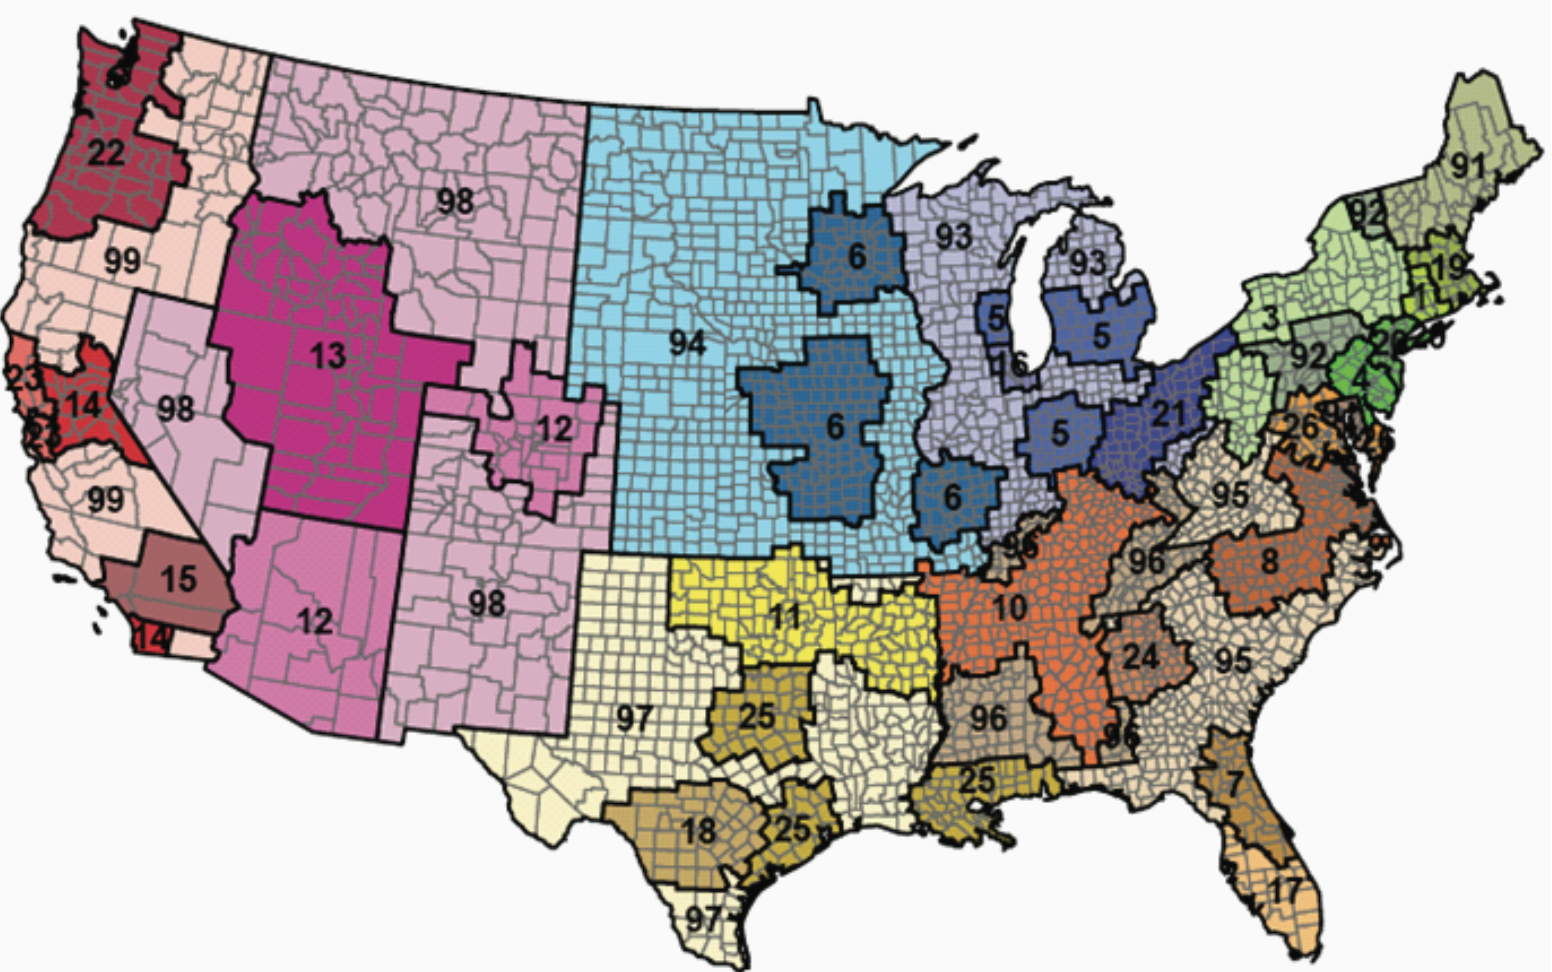
\includegraphics[width=\paperwidth]{./images/mktgrp_FPvary_map}}
            };
        \end{tikzpicture}
     \end{frame}
}

%%%%%OUR RESEARCH%%%%%%%%%%%%
\begin{frame}

\begin{center}\href{http://garretchristensen.shinyapps.io/Food_Price_Maps}{\beamergotobutton{QFAHPD Visualization}}

\vskip0.25in
\hrulefill

\vskip0.25in
Our data: At census block group level, but no map. 

Sorry!
\end{center}
\end{frame}

%%%%%%%%%%%%%%%%%%%%%%%%%%%%%%%%%%%%%%%%%%%%%%%%%%%%%%%%%%%%%%%%%%%%%%%%%%%%%%%%%%%%
\begin{frame}{FoodAPS}
``USDA's National Household Food Acquisition and Purchase Survey \href{https://www.ers.usda.gov/data-products/foodaps-national-household-food-acquisition-and-purchase-survey.aspx}{(FoodAPS)} is the first nationally representative survey of American households to collect unique and comprehensive data about household food purchases and acquisitions.''
\begin{itemize}
\item FoodAPS lets us look at the relationship between food prices and SNAP adequacy at a much finer geographical level.
\item  \href{https://www.ers.usda.gov/media/8612/priceindexdata.pdf}{Gunderson et al.} use IRI InfoScan data at store (or regional chain) level to build basketprice measure.
\item Index modeled after \href{https://www.cnpp.usda.gov/sites/default/files/usda_food_plans_cost_of_food/TFP2006Report.pdf}{Thrifty Food Plan} (TFP). 
\end{itemize}
\end{frame}





{
   \setbeamertemplate{navigation symbols}{}
    \begin{frame}[plain]
        \begin{tikzpicture}[remember picture,overlay]
            \node[at=(current page.center)] {
                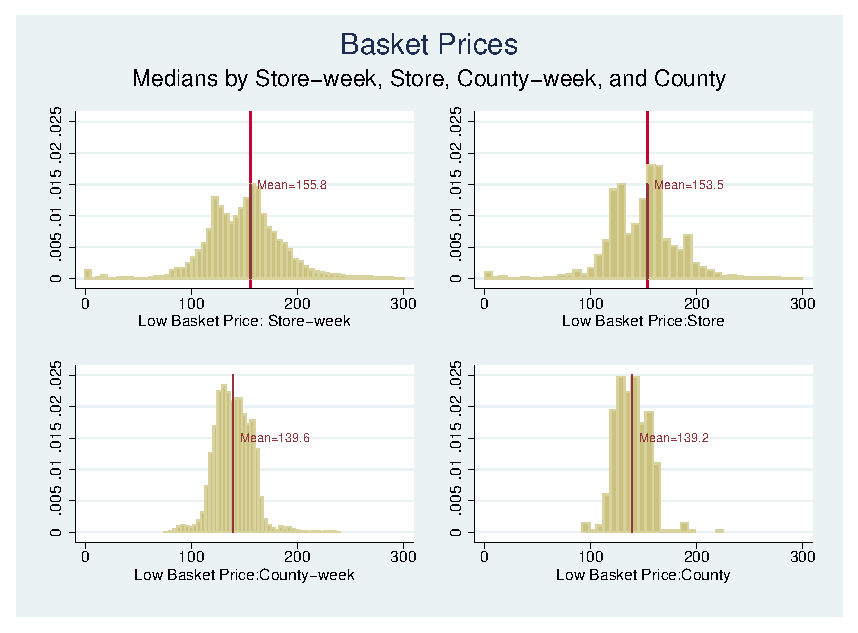
\includegraphics[height=\paperheight]{./images/ComboBPHisto.eps}
            };
        \end{tikzpicture}
     \end{frame}
}

\begin{frame}{The Thrifty Food Plan (TFP)}
  \setlength{\leftmargini}{1em}
\begin{itemize}
\item
Well-defined basket of foods to obtain a nutritious diet at a minimal cost.

\item
You're supposed to be able to buy TFP with 30\% of net income + food stamp benefits.

\item That's where the 649 comes from: $ Benefits=MaxBenefits(\$649/month)-NetIncome*0.3 $
\end{itemize}
\end{frame}


%\begin{frame}
%\begin{figure}
%\frame{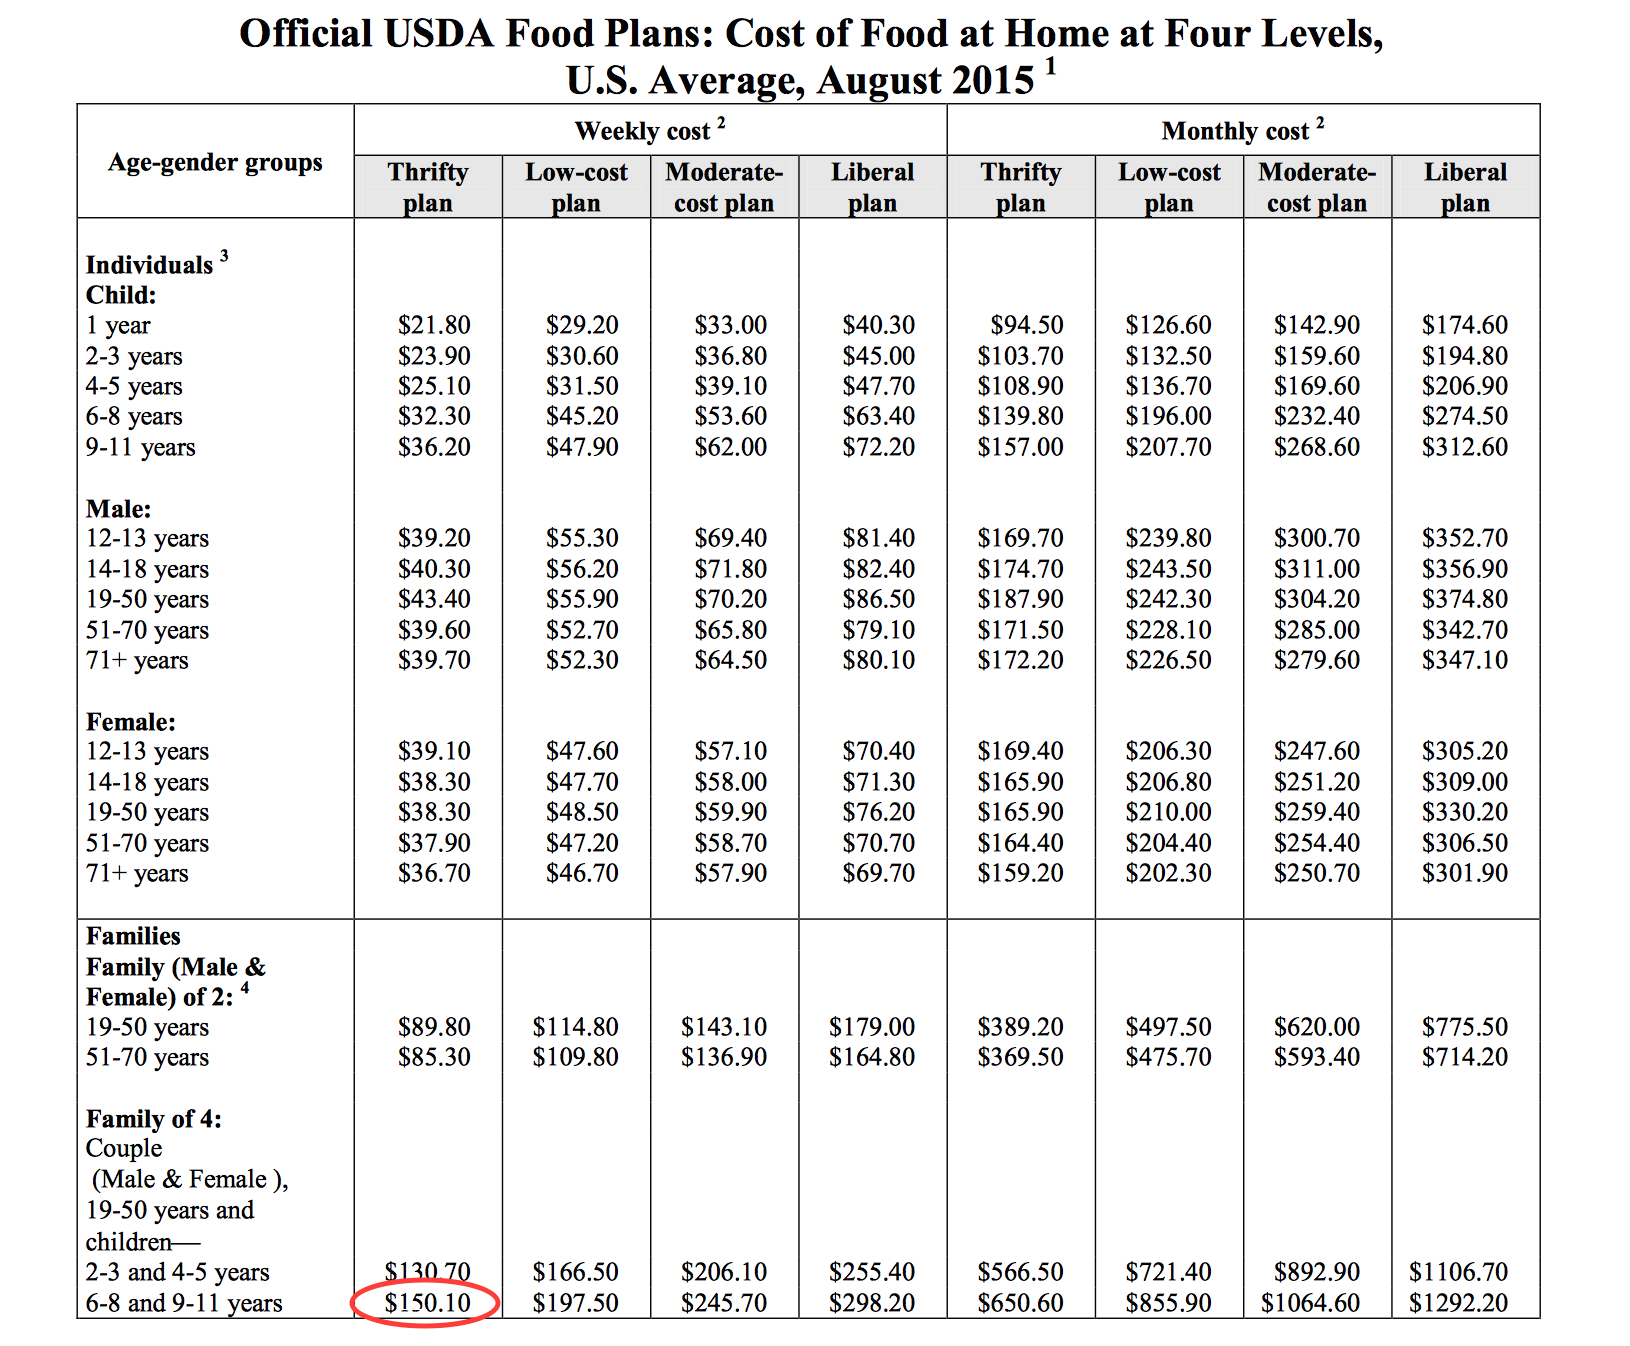
\includegraphics[scale=0.35]{./images/TFPa}}
%\end{figure}
%\end{frame}
%%%%%%%%%%%%%%%%HISTOGRAMS OF TFP

%\begin{frame}
%\begin{figure}
%{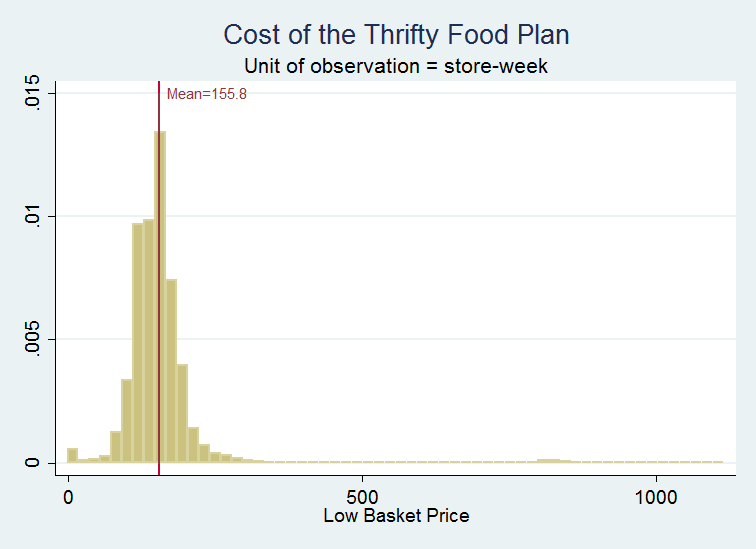
\includegraphics[scale=.4, trim=0cm .0cm 0cm 0cm, clip=true]{./images/low_basket_price_histo.png}}
%\end{figure}
%\end{frame}
%%%%%%%%%%%%%%%%%%%%%%%%%%%


\begin{frame}{SNAP Sufficiency for TFP}
 \large{Are SNAP benefits adequate for SNAP households to purchase the TFP? If not, what is the shortfall?}\\
\vskip6pt \hspace{2mm} \normalsize{\underline{\textit{Compare TFP cost to:}}}
\begin{itemize}
{\item SNAP benefit received + 30\% of net income} 
{\item Legislated maximum SNAP benefit} 
\end{itemize}
%{\item \vskip12pt \large{What about for SNAP-eligible households?}}\\
%{\item \vskip12pt \large{For which types of households are SNAP benefits inadequate?}}

\end{frame}

%%%%%%%%%%%%%%%%%%%%%%%%%%%%%%%%%%%%%%%%%%%%%%%%%%%%%%%%%%%%%%%%%%%%%%%%%%%%%%%%%%%
\begin{frame}

% Table generated by Excel2LaTeX from sheet 'Tcounty-st-cr-suff'
\begin{table}[htbp]{Sufficiency Rates of SNAP for Recipient Households by Distance from Stores}

\begin{adjustbox}{height=1.5in}
  \centering
    \begin{tabular}{llllll}
    \toprule
          & Average  & N     & Average  & N \\

     & \multicolumn{2}{l}{Net Income} & \multicolumn{2}{l}{Max Benefits} \\

    \midrule
    Census Region Median & 78\%    & 1444  & 83\%    & 1581 \\
    State Median & 79\%    & 1444  & 76\%    & 1581 \\
    County Median & 79\%    & 1436  & 74\%    & 1572 \\
    20-mile Median & 78\%    & 1338  & 73\%    & 1464 \\
    10-mile Median & 78\%    & 1311  & 73\%    & 1433 \\
    5-mile Median & 77\%    & 1224  & 72\%    & 1338 \\
    3.4-mile Median & 77\%    & 1174  & 74\%    & 1281 \\
    2.5mile Median & 77\%    & 1123  & 72\%    & 1225 \\
    10-nearest Median & 79\%    & 1338  & 77\%    & 1464 \\
    5-nearest Median & 78\%    & 1332  & 71\%    & 1458 \\
      \bottomrule
    \end{tabular}
    \end{adjustbox}
	\end{table}

\end{frame}

\begin{frame}

% Table generated by Excel2LaTeX from sheet 'Tcounty-st-cr-suff'
\begin{table}[htbp]{Sufficiency Rates of SNAP for Recipient Households by Distance from Stores}

\begin{adjustbox}{height=1.5in}
  \centering
    \begin{tabular}{llllll}
    \toprule
          & Average  & N     & Average  & N \\

     & \multicolumn{2}{l}{Net Income} & \multicolumn{2}{l}{Max Benefits} \\

    \midrule
    Census Region Minimum & 100\%  & 1444  & 100\%   & 1581 \\
    State Minimum & 99\%   & 1444  & 100\%   & 1581 \\
    County Minimum & 94\%   & 1436  & 100\%   & 1572 \\
    20-mile Minimum & 95\%    & 1338  & 100\%   & 1464 \\
    10-mile Minimum & 93\%    & 1311  & 100\%   & 1433 \\
    5-mile Minimum & 91\%    & 1224  & 99\%    & 1338 \\
    3.4-mile Minimum & 90\%    & 1174  & 100\%   & 1281 \\
    2.5mile Minimum & 90\%    & 1123  & 99\%    & 1225 \\
    10-nearest Minimum & 91\%    & 1338  & 100\%   & 1464 \\
    5-nearest Minimum & 89\%    & 1332  & 98\%    & 1458 \\
    2-nearest Minimum & 83\%    & 1332  & 85\%    & 1458 \\
    \bottomrule
    \end{tabular}
    \end{adjustbox}
	\end{table}

\end{frame}
%%%%%%%%%%%%%%%%%%%%%%%%%%%%%%%%%%%%%%%%%%%%%%%%%%%%%%%%%%%%%%%%%%%%%%%%%%%%
%%%%%%%%%%%%%%%%%%%%%%%%%%%%%%%%%%%%%%%%%%%%%%%%%%%%%%%%%%%%%%%%%%%%%%%%%
%\begin{frame}
%\begin{figure}
%{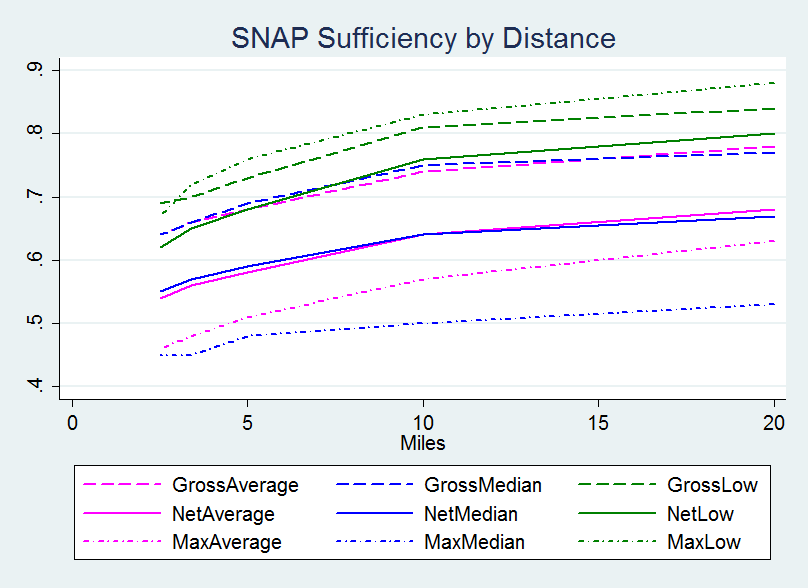
\includegraphics[scale=.4, trim=0cm .0cm 0cm 0cm, clip=true]{./images/quicklinegraph.png}}
%\end{figure}
%\end{frame}

%%%%%%%%%%%%%%%%%%%%%%%%%%%%%%%%%%%%%%%%%%%%%%%%%%%%%%%%%%%%%%%%%%%%%%%%


%%%%%%%%%%%%%%%%%%%%%%%%%%%%%%%%%%%%%%%%%%%%%%%%%%%%%%%%%%%%%%%%%%%%%%%%%%%%%%%%%%%%%%%%%%
\begin{frame}
% Table generated by Excel2LaTeX from sheet 'Tcharacteristics'
\begin{table}{Characteristics of Households by SNAP Sufficiency}%[htbp]

\begin{adjustbox}{max width=\textwidth}
  \centering
  %\caption{}
     \begin{tabular}{lllllll}
    \toprule
    & \multicolumn{3}{l}{SNAP Recipients} & \multicolumn{3}{l}{SNAP Eligible} \\

    Characteristic & No    & Yes   & P-value & No    & Yes   & P-value \\
    \midrule
    Family Size & 2.78  & 2.65  & 0.43  & 2.52  & 2.21  & 0.11 \\
    Household Max Age & 50.83 & 49.35 & 0.30  & 53.22 & 53.00 & 0.89 \\
    Household Min Age & 27.00 & 28.14 & 0.65  & 34.82 & 37.21 & 0.43 \\
    \textbf{Household Income $(\$1K)$} & 2392 & 1950 & 0.05  & 3059 & 2355 & 0.04 \\
    Percent of Poverty Line & 141.95 & 124.20 & 0.12  & 209.82 & 172.74 & 0.08 \\
    HH Has Earned Income & 0.50  & 0.53  & 0.57  & 0.60  & 0.55  & 0.21 \\
    Household Max Education & 20.08 & 19.65 & 0.10  & 20.76 & 20.24 & 0.09 \\
    HH Has Elderly Member & 0.30  & 0.27  & 0.40  & 0.38  & 0.37  & 0.83 \\
      \textbf{Metro Area} & 0.97  & 0.83  & 0.01  & 0.97  & 0.83  & 0.02 \\
    High Food Security & 0.34  & 0.32  & 0.52  & 0.45  & 0.50  & 0.44 \\
    Marginal Food Security & 0.25  & 0.21  & 0.24  & 0.23  & 0.19  & 0.13 \\
    Low Food Security & 0.24  & 0.26  & 0.57  & 0.21  & 0.16  & 0.08 \\
    Very Low Food Security & 0.18  & 0.21  & 0.40  & 0.11  & 0.16  & 0.02 \\
    Trouble Paying Bills & 0.30  & 0.27  & 0.45  & 0.18  & 0.17  & 0.83 \\
    High Price Area & 0.88  & 0.00  & 0.00  & 0.90  & 0.00  & 0.00 \\
    Northeast & 0.22  & 0.09  & 0.25  & 0.29  & 0.09  & 0.13 \\
    Midwest & 0.24  & 0.34  & 0.33  & 0.16  & 0.35  & 0.05 \\
    South & 0.33  & 0.43  & 0.25  & 0.32  & 0.42  & 0.33 \\
    West  & 0.21  & 0.14  & 0.49  & 0.22  & 0.14  & 0.39 \\

    
    \bottomrule
\end{tabular}
\end{adjustbox}
\end{table}
\end{frame}


%%%%%%%%%%%%%%%%%%%%%%%%%%%%%%%%%%%%%%%%%%%%%%%%%%%%%%%%%%%%%%%%%%%%%%%%%

%%%%%%%%%%%%%%%%%%%%%%%%%%%%%%%%%%%%%%%%%%%%%%%%
\begin{frame}{Nutrition: Overview}
\begin{itemize}
\item Use local relative generosity of SNAP to measure nutrition impacts.
\item Cross-sectional data: use \href{http://www.tandfonline.com/doi/abs/10.1080/07350015.2016.1227711}{Oster's 2016} improvement to \href{http://www.journals.uchicago.edu/doi/abs/10.1086/426036}{Altonji, Elder, Taber 2005} method to compare with and without observable controls.
\item National School Lunch Program and the School Breakfast Program as mediators.
\item Outcomes:
\begin{itemize}
\item Healthy Eating Index (total, fruit, veg)
\item Percent of calories from added sugar, solid fat, alcohol %(sofa\_perc)
\item Alcohol (Grams)
\item Self-reported nutrition status
\end{itemize}
\end{itemize}

\end{frame}


%%%%%%%%%%%%%%%%%%%%%%%%%%%%%%%%%%%%%%%%%%%

\begin{frame}{Healthy Eating Index}

\begin{itemize}
\item 
 Created by USDA's Center for Nutrition Policy and Promotion (CNPP) to assess conformance to the \textit{Dietary Guidelines for Americans}. Updated every five years. \href{https://www.cnpp.usda.gov/sites/default/files/healthy_eating_index/HEI2010-UpdatePaper.pdf}{(Guenther et al.)}. 
\item Valid for age $>2$.
\item 
Nine adequacy, three moderation components.
\item 
Density approach (per 1000 calories).
\item 
Zeros prevalent in component scores.
\item 
National average ~60/100. 
\end{itemize}
\end{frame}

\begin{frame}{Healthy Eating Index}
\begin{table}{}
\begin{tabular}{lll}

HEI-2010 Dietary Component & Max Score & Moderation \\
\toprule
Total Fruit & 5 & \\
Whole Fruit & 5 & \\
Total Vegetables & 5& \\
Greens and Beans & 5 &\\
Whole Grains & 10 &\\
Dairy & 10& \\
Total Protein Foods & 5& \\
Seafood and Plant Proteins & 5& \\
Fatty Acids & 10& \\
Refined Grains & 10& M \\
Sodium & 10 & M\\
Empty Calories & 20&  M \\
\bottomrule 
\end{tabular}
\end{table}
\begin{tiny}\begin{center}
Note: See \href{https://www.cnpp.usda.gov/sites/default/files/healthy_eating_index/CNPPFactSheetNo2.pdf}{CNPP factsheet} for scoring standards. \end{center}\end{tiny}
\end{frame}


\begin{frame}{Nutrition: Controlling for Observables}
 $$Nutrition_{ij}=\alpha + \beta \cdot f(TFP_{ij}, MAXSNAP_{ij}) + X_{ij} \cdot \theta + \delta_{j}+\epsilon_{ij} $$
 
\begin{itemize}
\item Focus on $log(SNAPMAX_{ij}/TFP_{ij})$ as independent variable of interest, though it could be $log (TFP_{ij})$, sufficiency[0/1], or gap[continuous].
\item $X$ is rural, metro, income, trouble with bills, large expenditure, household size, car ownership, tobacco use, days since SNAP receive, WIC eligibility, WIC use, age, race, sex, non-food CPI (9).
\item State fixed effects
\end{itemize}
\end{frame}

\begin{frame}{Methods: Controlling for Observables}
\begin{itemize}
\item Individual level
\begin{itemize}
\item Assume FAH consumed by all, assign FAFH to individual
\end{itemize}
\item Primary sample: SNAP participants
\begin{itemize}
\item Children and adults separately
\end{itemize}
\item Placebo: $>300\%$ Federal 
\item Regressions weighted according to complex survey design. \begin{tiny}\href{https://www.ers.usda.gov/media/8804/0_foodaps-user-guide-puf.pdf}{User's Guide Pg 55}\end{tiny}
\end{itemize}
\end{frame}

\begin{frame}{Methods: Oster 2016}

$$Y=\beta X +\Psi \omega^0+W_2+\epsilon$$

$X$ is treatment of interest.

$\omega$ observed, W is not.
\vskip0.1in
What happens to our effect estimate if we assume the unobservables have a similar correlation to treatment as the observables?
\vskip0.1in
Depends on relative degree of selection on observed and unobserved variables $(\delta)$, as well as $R^2$ resulting from controlling for unobservables, $R_{max}$.
\end{frame}

\begin{frame}{Oster 2016}
\href{http://jhr.uwpress.org/content/XL/4/791.short}{Altonji, Elder, Taber (2005)} implicitly assume $R_{max}$=1. Perhaps unlikely due to measurement error or idiosyncratic variation.
\vskip0.1in
\href{http://www.sciencedirect.com/science/article/pii/S0047272709000942}{Bellows \& Miguel 2009}, \href{https://www.aeaweb.org/articles?id=10.1257/aer.101.7.3221}{Nunn \& Wantchekon 2011} assume $R_{max}=\tilde{R}+(\tilde{R}-\mathring{R})$. 
\vskip0.1in
$R_{max}$ is a flexible parameter in Oster's method, but $1.3\times\tilde{R}$ performs well in tests.
\vskip0.1in
$$\beta^* \approx \tilde{\beta}-\delta(\mathring{\beta}-\tilde{\beta})\frac{R_{max}-\tilde{R}}{\tilde{R}-\mathring{R}}$$ 

\end{frame}

{
   \setbeamertemplate{navigation symbols}{}
    \begin{frame}[plain]
        \begin{tikzpicture}[remember picture,overlay]
            \node[at=(current page.center)] {
                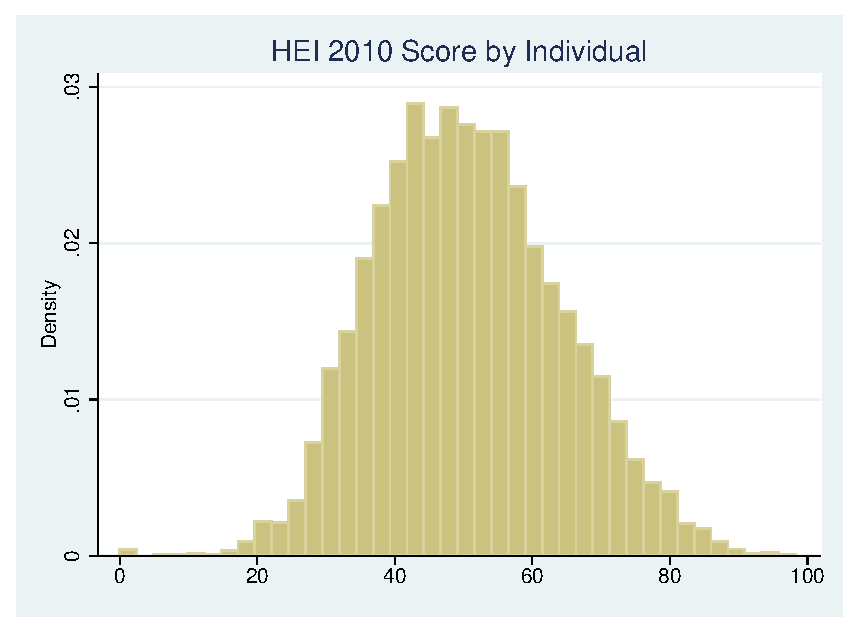
\includegraphics[height=\paperheight]{./images/HEI_Itotalscore.eps}
            };
        \end{tikzpicture}
     \end{frame}
}
{
   \setbeamertemplate{navigation symbols}{}
    \begin{frame}[plain]
        \begin{tikzpicture}[remember picture,overlay]
            \node[at=(current page.center)] {
                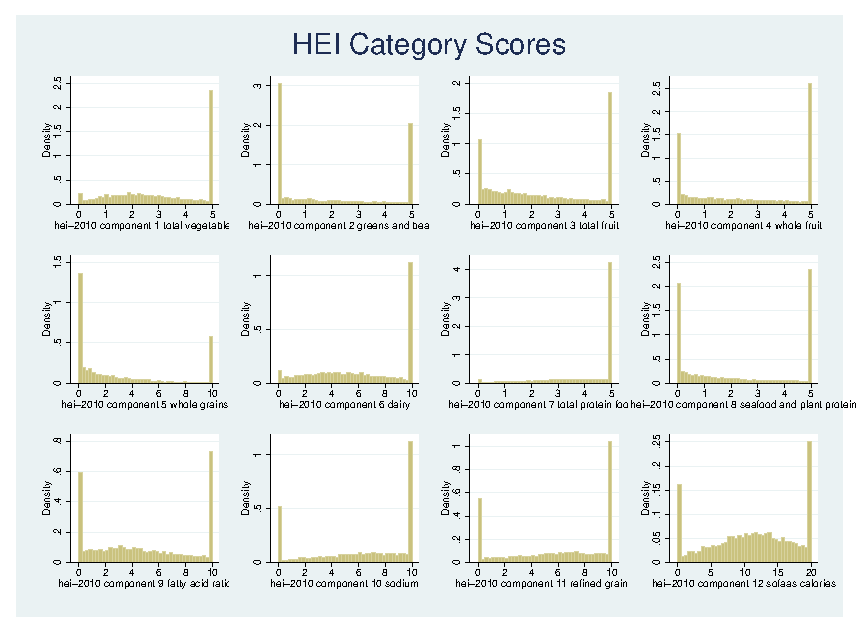
\includegraphics[height=\paperheight]{./images/HEI_Iscore_combined.eps}
            };
        \end{tikzpicture}
     \end{frame}
}
{
   \setbeamertemplate{navigation symbols}{}
    \begin{frame}[plain]
        \begin{tikzpicture}[remember picture,overlay]
            \node[at=(current page.center)] {
                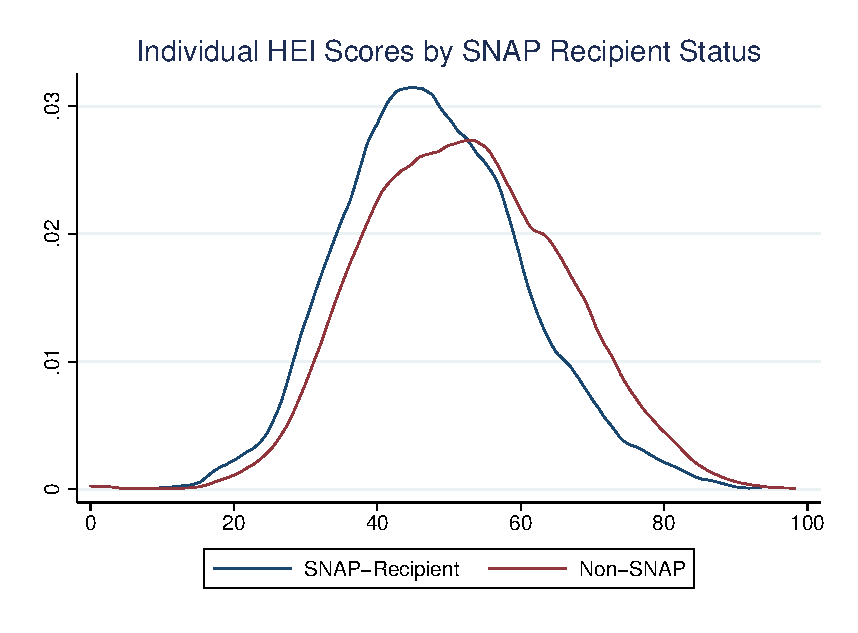
\includegraphics[height=\paperheight]{./images/HEI_Idensity.eps}
            };
        \end{tikzpicture}
     \end{frame}
}
{
   \setbeamertemplate{navigation symbols}{}
    \begin{frame}[plain]
        \begin{tikzpicture}[remember picture,overlay]
            \node[at=(current page.center)] {
                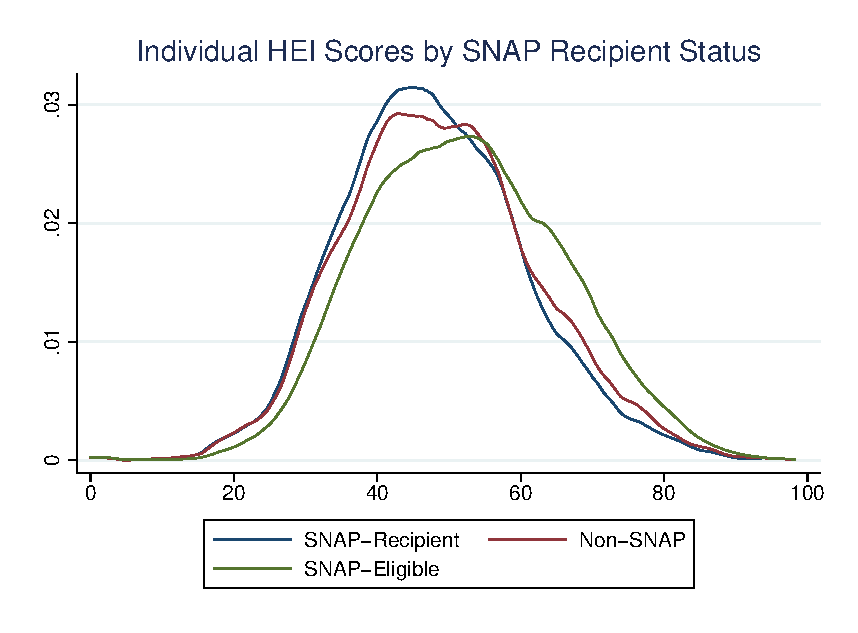
\includegraphics[height=\paperheight]{./images/HEI_Idensity3.eps}
            };
        \end{tikzpicture}
     \end{frame}
}
{
   \setbeamertemplate{navigation symbols}{}
    \begin{frame}[plain]
        \begin{tikzpicture}[remember picture,overlay]
            \node[at=(current page.center)] {
                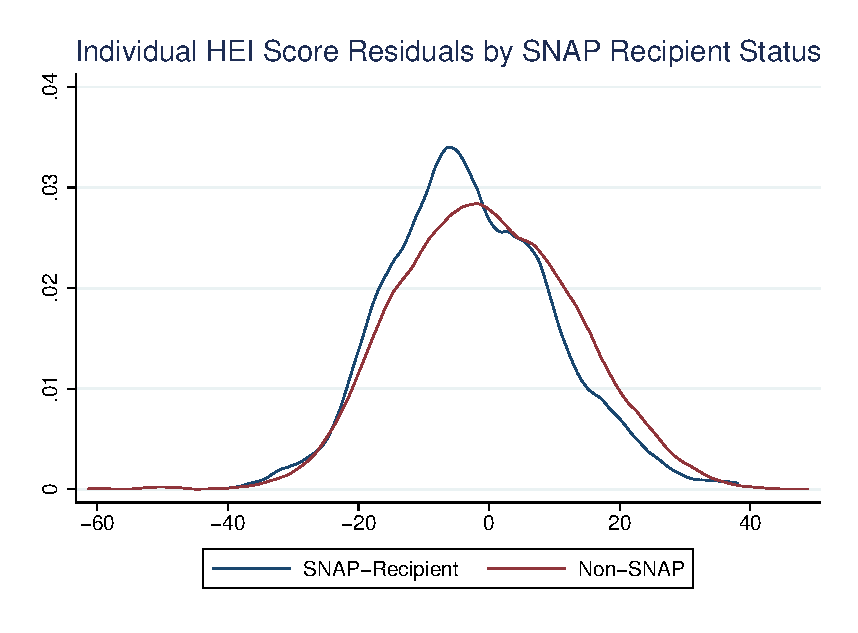
\includegraphics[height=\paperheight]{./images/HEI_IdensityResid.eps}
            };
        \end{tikzpicture}
     \end{frame}
}
{
   \setbeamertemplate{navigation symbols}{}
    \begin{frame}[plain]
        \begin{tikzpicture}[remember picture,overlay]
            \node[at=(current page.center)] {
                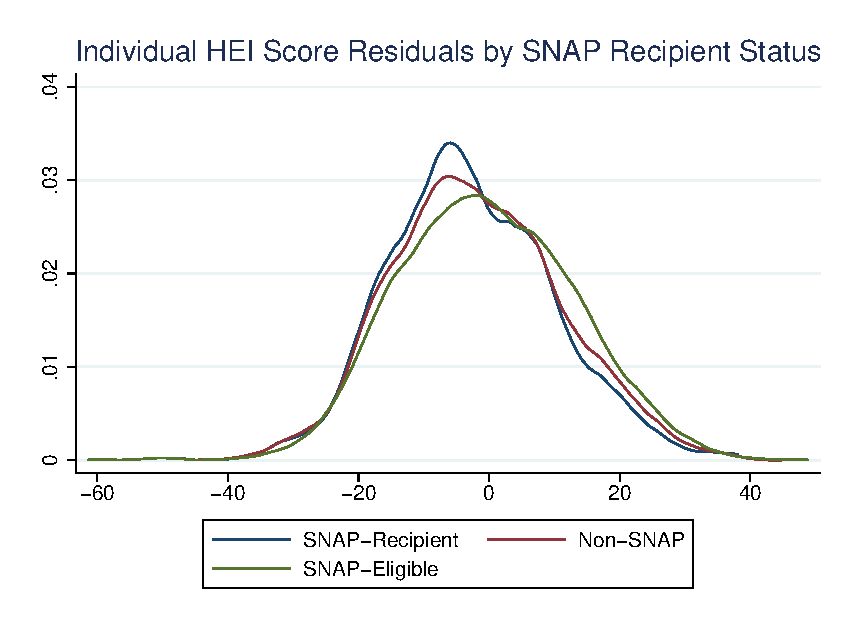
\includegraphics[height=\paperheight]{./images/HEI_Idensity3Resid.eps}
            };
        \end{tikzpicture}
     \end{frame}
}

%%%%%%%%%%%%%%%%%%%%%%%%%%%%%%%%%%%%%%%%
%\begin{frame}{Results}
%\begin{table}{HEI Total Score: SNAP All Individuals}
%
%\begin{tabular}{llll}
%\toprule
%& (1) & (2) & (3) \\
%\midrule
%ln(SNAPMAX/TFP) & -5.031 & 8.630* & 13.24 \\
%& (4.255) & (4.696) & (9.123) \\
%\\
%N & 3620 & 3551 & 3551 \\
%$R^2$ & 0.002 & 0.120 & 0.160 \\
%Mean & 53.25 & 53.25 & 53.25 \\
%Effect10 & -0.480 & 0.823 & 1.262 \\
%Beta($R_{max}=1)$&  & 158.7 & 136.5 \\
%Delta($R_{max}=1)$&  & -0.0345 & -0.0642 \\
%Beta($R_{max}=1.3\tilde{R})$ &  & 16.63 & 22 \\
%Delta($R_{max}=1.3\tilde{R})$&  & -0.752 & -0.923 \\
%Controls & & YES & YES \\
%State FE &  &  & YES \\
%\bottomrule
%
%\end{tabular}
%\end{table}
%\end{frame}
%
%\begin{frame}{Results}
%\begin{table}{Nutrition Outcomes: SNAP All Individuals}
%\begin{tabular}{llll}
%\toprule
%& (1) & (2) & (3)   \\
%
%& HEI-Veg & HEI-Fruit & SOFA   \\
%\midrule
%\\
%ln(SNAPMAX/TFP) & 1.526 & 0.555 & -7.739   \\
%& (0.926) & (1.191) & (6.626)  \\
%\\
%N & 3851 & 3851 & 3851   \\
%$R^2$ & 0.085 & 0.154 & 0.127   \\
%Mean & 3.205 & 2.580 & 31.75   \\
%Effect10 & 0.145 & 0.0529 & -0.738   \\
%Beta($R_{max}=1.3\tilde{R})$ & 2.317 & 1.449 & -13.10   \\
%Delta($R_{max}=1.3\tilde{R})$ & -0.966 & -0.619 & -1.140   \\
%Controls & YES & YES & YES   \\
%State FE & YES & YES & YES   \\
%\bottomrule
%\end{tabular}
%\end{table}
%\end{frame}
%
%\begin{frame}{Results}
%\begin{table}{Nutrition Outcomes: FPL$>300$\%FPL All Individuals}
%\begin{adjustbox}{max width=\textwidth}
%\centering
%\begin{tabular}{llllll}
%\toprule
%& (1) & (2) & (3) & (4) & (5) \\
%& HEI Total & HEI Veg & HEI Fruit & SOFA & Alcohol \\
%\midrule
%\\
%ln(SNAPMAX/TFP) & -34.45 & -0.113 & -1.159 & 7.891 & -21.05 \\
%& (50.43) & (3.927) & (4.500) & (16.79) & (456.2) \\
%\\
%N & 230 & 257 & 257 & 257 & 257 \\
%$R^2$ & 0.442 & 0.535 & 0.477 & 0.364 & 0.421 \\
%Mean & 53.02 & 3.205 & 2.565 & 31.81 & 67.22 \\
%Effect10 & -3.284 & -0.0108 & -0.110 & 0.752 & -2.006 \\
%Beta($R_{max}=1.3\tilde{R}$)& -42.51 & 0.101 & -0.970 & 7.848 & -20.99 \\
%Delta($R_{max}=1.3\tilde{R}$)& -3.255 & 0.538 & 4.922 & 20.06 & 22.47 \\
%Controls & YES & YES & YES & YES & YES \\
%State FE & YES & YES & YES & YES & YES \\
%\bottomrule
%\end{tabular}
%\end{adjustbox}
%\end{table}
%\end{frame}
%%%%%%%%%%%%%%%%%%%%%%%%%%%%%%%%%%%%%
\begin{frame}
\begin{table}{HEI Total: SNAP Children 2-17}
\begin{adjustbox}{max width=\textwidth}
\begin{tabular}{lllll}
\toprule

 & (1) & (2) & (3) & (4) \\
\midrule
 \\
ln(SNAPMAX/TFP) & -2.938 & 11.55* & 18.17 & 20.65* \\
 & (6.426) & (5.919) & (12.54) & (11.35) \\
School Breakfast &  &  &  & 1.020 \\
 &  &  &  & (2.757) \\
School Lunch &  &  &  & -4.482 \\
 &  &  &  & (6.768) \\
 \\
N & 990 & 975 & 975 & 842 \\
$R^2$ & 0.001 & 0.160 & 0.225 & 0.296 \\
Mean & 53.11 & 53.11 & 53.11 & 53.13 \\
Effect10 & -0.280 & 1.100 & 1.731 & 1.968 \\
Beta($R_{max}=1)$ &  & 141.4 & 118.6 & 116.1 \\
Delta($R_{max}=1)$ &  & -0.0600 & -0.115 & -0.177 \\
Beta($R_{max}=1.3\tilde{R})$ &  & 20.26 & 28.14 & 32.63 \\
Delta($R_{max}=1.3\tilde{R})$ &  & -0.904 & -1.044 & -1.139 \\
Controls & NO & YES & YES & YES \\
State FE &  &  & YES & YES \\

\end{tabular}
\end{adjustbox}
\end{table}
\end{frame}


\begin{frame}
\begin{table}{Nutrition Outcomes: SNAP Children 2-17}
\begin{adjustbox}{max width=\textwidth}
\begin{tabular}{llll}
\toprule
 & (1) & (2) & (3) \\
 & HEI Veg & HEI Fruit & SOFA \\
\midrule
 \\
ln(SNAPMAX/TFP) & 1.751 & 1.102 & -11.90 \\
 & (1.272) & (1.632) & (12.11) \\
 \\
N & 1065 & 1065 & 1065 \\
$R^2$ & 0.201 & 0.158 & 0.230 \\
Mean & 3.201 & 2.573 & 31.79 \\
Effect10 & 0.167 & 0.105 & -1.134 \\
Beta$(R_{max}=1.3\tilde{R})$ & 2.672 & 2.121 & -18.64 \\
Delta$(R_{max}=1.3\tilde{R})$ & -1.500 & -0.941 & -1.387 \\
Controls & YES & YES & YES \\
State FE & YES & YES & YES \\
\bottomrule
\end{tabular}
\end{adjustbox}
\end{table}
\end{frame}

\begin{frame}
\begin{table}{Nutrition Outcomes:$>300\%$ FPL Children 2-17---Placebo Sample}
\begin{adjustbox}{max width=\textwidth}

\begin{tabular}{llllll}
\toprule
 & (1) & (2) & (3) & (4) & (5) \\
 & HEI Total & HEI Veg & HEI Fruit & SOFA & Alcohol \\
 \midrule
 \\
ln(SNAPMAX/TFP) & -34.45 & -0.113 & -1.159 & 7.891 & -21.05 \\
 & (50.43) & (3.927) & (4.500) & (16.79) & (456.2) \\
 \\
 N & 230 & 257 & 257 & 257 & 257 \\
$R^2$ & 0.442 & 0.535 & 0.477 & 0.364 & 0.421 \\
Mean & 53.02 & 3.205 & 2.565 & 31.81 & 67.22 \\
Effect10 & -3.284 & -0.0108 & -0.110 & 0.752 & -2.006 \\
Beta$(R_{max}=1.3\tilde{R})$  & -42.51 & 0.101 & -0.970 & 7.848 & -20.99 \\
Delta$(R_{max}=1.3\tilde{R})$  & -3.255 & 0.538 & 4.922 & 20.06 & 22.47 \\
Controls & YES & YES & YES & YES & YES \\
State FE & YES & YES & YES & YES & YES \\
\bottomrule
\end{tabular}


\end{adjustbox}
\end{table}
\end{frame}


%%%%%%%%%%%%%%%%%%%%%%%%%%%%%%%%%%%%
\begin{frame}{Results}
\begin{table}{Nutrition Outcomes: SNAP Adults}
\begin{adjustbox}{max width=\textwidth}
\begin{tabular}{llllll}
\toprule
 & (1) & (2) & (3) & (4) & (5) \\
 & HEI Total & HEI Veg & HEI Fruit & SOFA & Alcohol \\
\midrule
 \\
ln(SNAPMAX/TFP) & 10.27 & 1.475 & 0.401 & -8.201 & -21.38 \\
 & (10.49) & (1.062) & (1.188) & (6.069) & (83.26) \\
 \\
Observations & 2145 & 2311 & 2311 & 2311 & 2311 \\
R-squared & 0.168 & 0.089 & 0.176 & 0.127 & 0.066 \\
Mean & 53.18 & 3.206 & 2.589 & 31.78 & 67.97 \\
Effect10 & 0.978 & 0.141 & 0.0382 & -0.782 & -2.038 \\
Beta($R_{max}=1.3\tilde{R}$) & 18.42 & 2.235 & 1.217 & -13.44 & -17.95 \\
Delta($R_{max}=1.3\tilde{R}$) & -0.909 & -1.027 & -0.501 & -1.166 & 4.310 \\
Controls & YES & YES & YES & YES & YES \\
State FE & YES & YES & YES & YES & YES \\
\bottomrule
\end{tabular}
\end{adjustbox}
\end{table}
\end{frame}


\begin{frame}{Results}
\begin{table}{Obesity: SNAP Adults}
\begin{adjustbox}{max width=\textwidth}
\begin{tabular}{lllllll}
\toprule
 & \multicolumn{3}{c}{Obese} & \multicolumn{3}{c}{Overweight} \\
 & (1) & (2) & (3) & (4) & (5) & (6) \\
\midrule
 \\
ln(SNAPMAX/TFP) & 0.367*** & 0.352*** & 0.422* & 0.0644 & 0.120* & 0.106 \\
 & (0.121) & (0.102) & (0.248) & (0.0846) & (0.0654) & (0.171) \\
 \\
Observations & 2350 & 2289 & 2289 & 2350 & 2289 & 2289 \\
R-squared & 0.008 & 0.074 & 0.106 & 0.000 & 0.062 & 0.093 \\
Mean & 0.280 & 0.280 & 0.280 & 0.581 & 0.581 & 0.581 \\
Effect10 & 0.0350 & 0.0335 & 0.0402 & 0.00614 & 0.0115 & 0.0101 \\
Beta($R_{max}=1.3\tilde{R}$) &  & 0.407 & 0.503 &  & -2.419 & -0.225 \\
Delta($R_{max}=1.3\tilde{R}$) &  & -10.69 & -6.547 &  & -0.389 & 0.383 \\
Controls &&YES &YES &&YES & YES\\
State FE &  &  & YES &  &  & YES \\
\bottomrule
\end{tabular}

\end{adjustbox}
\end{table}
\end{frame}
%%%%%%%%%%%%%%%%%%%%%%%%%%%%%%%%%%%%%%%%%%%%%
\begin{frame}{Nutrition}
Tentative conclusions
 
\begin{itemize}
\item Some suggestive evidence of improvements in HEI with higher SNAP purchasing power.
\item Sign indicates more fruit and vegetables, less sugar, fat, and alcohol.
\item Similar (insignificant) HEI  results in children and adults.
\item Significantly higher obesity among SNAP recipient adults with higher SNAP purchasing power.
\end{itemize}
\end{frame}
%%%%%%%%%%%%%%%%%%%%%%%%%%%%%%%%%%%%%%%%%%%%%%%%%%%%%
\begin{frame}[plain]
\hspace{34mm}
\color{blue!60!black!60}{\Huge{Thank You}}
\end{frame}

\end{document}


